\documentclass[25pt, a0paper, landscape, margin=0mm, innermargin=20mm,
blockverticalspace=2mm, colspace=20mm, subcolspace=0mm]{tikzposter} %Default values for poster format options.

\input{packages}
\input{style}

\begin{document}

\renewcommand{\baselinestretch}{1}
\title{\parbox{1900pt}{Pushing the limits of time-frequency uncertainty in the
detection of transient communication signals in weakly electric fish}}
\author{Sina Prause, Alexander Wendt, Patrick Weygoldt}
\institute{Supervised by Till Raab \& Jan Benda, Neurothology Group,
University of Tübingen}
\usetitlestyle[]{sampletitle}
\maketitle
\renewcommand{\baselinestretch}{1.4}

\begin{columns}
\column{0.5}
\myblock[TranspBlock]{Introduction}{
    \begin{minipage}[t]{0.55\linewidth}
        The time-frequency tradeoff makes reliable signal detecion and simultaneous
        sender identification of freely interacting individuals impossible.
        This profoundly limits our current understanding of chirps to experiments
        with single - or physically separated - individuals.
    \end{minipage} \hfill
    \begin{minipage}[t]{0.40\linewidth}
    \vspace{-1.5cm}
    \begin{tikzfigure}[]
        \label{tradeoff}
        \includegraphics[width=\linewidth]{example-image-a}
    \end{tikzfigure}
    \end{minipage}
}

\myblock[TranspBlock]{A chirp detection algorithm}{
    \begin{minipage}[t]{0.55\linewidth}
        \vspace{-1.5cm}
        \begin{tikzfigure}[]
            \label{modulations}
            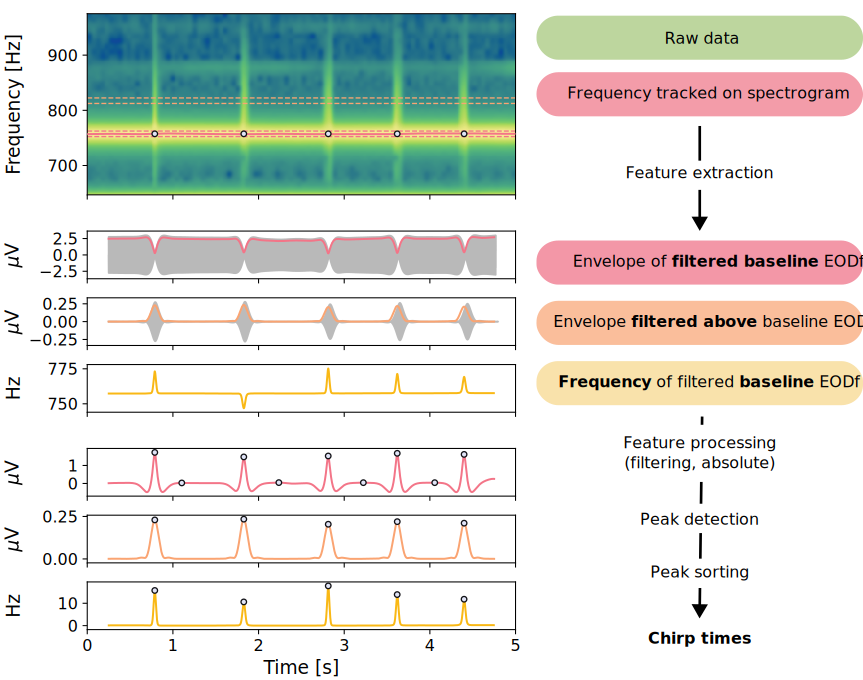
\includegraphics[width=\linewidth]{figs/10.0_11245.5.pdf}
        \end{tikzfigure}
    \end{minipage} \hfill
    \begin{minipage}[t]{0.40\linewidth}
            \lipsum[3][1-5]
    \end{minipage}
}

\column{0.5}
\myblock[TranspBlock]{Results}{
    \lipsum[3][1-5]
    \begin{tikzfigure}[]
        \label{modulations}
        \includegraphics[width=\linewidth]{example-image-c}
    \end{tikzfigure}
}

\myblock[TranspBlock]{More Stuff}{
    \lipsum[3][1-9]
}

% \column{0.3}
% \myblock[TranspBlock]{More Results}{
%     \begin{tikzfigure}[]
%         \label{results}
%         \includegraphics[width=\linewidth]{example-image-a}
%     \end{tikzfigure}

%     \begin{multicols}{2}
%     \lipsum[5][1-8]
%     \end{multicols}
%     \vspace{-1cm}
% }

% \myblock[TranspBlock]{Conclusion}{
%     \begin{itemize}
%         \setlength\itemsep{0.5em}
%         \item \lipsum[1][1]
%         \item \lipsum[1][1]
%         \item \lipsum[1][1]
%     \end{itemize}
%     \vspace{0.2cm}
%     }
\end{columns}

\node[
    above right,
    text=white,
    outer sep=45pt,
    minimum width=\paperwidth,
    align=center,
    draw,
    fill=boxes,
    color=boxes,
] at (-0.51\paperwidth,-43.5) {
\textcolor{text}{\normalsize Contact: \{name\}.\{surname\}@student.uni-tuebingen.de}};

\end{document}
